\documentclass[10pt,
%handout
aspectratio=169
]{beamer}
\usepackage[utf8]{inputenc}
\usepackage[T1]{fontenc}
\usepackage{lmodern}

\usepackage{nicefrac}
\usepackage{braket}

%\usepackage[backend=biber,style=chem-acs]{biblatex}
%\bibliography{biblio}


\usetheme{metropolis}
\setbeamercolor{block title}{use=structure,fg=white,bg=structure.fg!75!black}
\setbeamercolor{block body}{parent=normal text,use=block title,bg=block title.bg!10!bg}


\usepackage{tikz}
\usetikzlibrary{positioning, decorations.markings, decorations.pathmorphing, calc}

\usepackage{siunitx}
\usepackage{mhchem}
\usepackage{minted}
\setminted{  
	frame=lines,  
	framesep=2mm,  
	baselinestretch=1.2,  
	fontsize=\footnotesize,  
	linenos,  
	breaklines,
	tabsize=2
}  

\author{Pierre Beaujean (\href{mailto:pierre.beaujean@unamur.be}{pierre.beaujean@unamur.be})}
\title{Advanced Python for advanced users}
\subtitle{... And a few concepts of computer science}
\institute{University of Namur}
\date{March 2025 (version of  \today)}

\allowdisplaybreaks

\begin{document}
\begin{frame}[plain]
	\maketitle
\end{frame}

\begin{frame}{Table of content}
	\tableofcontents
\end{frame}

\section{Back to basics}

\begin{frame}{Computer?}
	As far as you are concerned, a computer contains:\begin{itemize}
		\item A \textbf{CPU}, which execute (\textit{assembler}) code. Nowadays, there are also \textbf{GPUs} which can fulfill this role.
		\item Different kind of \textbf{memories} (cache, RAM, disk, etc), some of which can be addressed differently (\textit{e.g.}, through files).
		\item Some interfaces to the outside world, via peripherics (screen,  mouse, Ethernet, etc).
	\end{itemize}
	
	By itself, the CPU only moves bytes around in memory, and can perform operation on them. It understands the concept of \textbf{integers} and \textbf{floating point numbers} (IEEE-754 shenanigans), but that's about it. 
	
	Most functionalities of a computer (\textit{e.g.}, files) are in fact available thanks to the \textbf{operating system}, which offers, \textit{e.g.}, an unified interface to peripherics.
\end{frame}

\begin{frame}
	The \textbf{assembler} is a pretty simple (and CPU-dependent) language. For example, it does not understand the concept of strings (which explains why Fortran and C implements them differently). And, among other things, \textit{advanced} concepts like \textit{loops} are not directly available.
	
	 So... A meme will now ensue.
	
	\begin{center}
		\includegraphics[width=.6\linewidth]{im/meme-goto}
		
		(Note: it is in fact \textbf{conditional jumps})
	\end{center}
\end{frame}

\begin{frame}{Programming in Python}
	A programming language enables you to express complex logic (\textit{e.g.}, loops, conditionals) in a structured and readable manner. This code is then either translated into machine instructions by a \textbf{compiler} or executed directly by an \textbf{interpreter}. While interpreted languages tend to be slower, they offer advantages such as dynamic execution (\mintinline{python}|exec()|), reflexivity (\mintinline{python}|getattr()|), and the ability to modify itself at runtime.
	
	Python is an \textbf{interpreted} language, but it is also \textit{just-in-time compiled} into an intermediate bytecode representation (stored in \mintinline{text}|__pycache__|). Over time, this process optimizes execution by reducing redundant checks, making subsequent runs of the code faster.
\end{frame}



\begin{frame}[fragile]
	The way to write the code is referred to as a \textbf{programming paradigm}, a relatively high-level way to conceptualize and structure the implementation of a computer program.\footnote{\url{https://en.wikipedia.org/wiki/Programming_paradigm}} Among others, there are:\begin{itemize}
		\item \textbf{Imperative}, in which the code directly controls execution flow and state change. This includes the famous \textbf{procedural} (\mintinline{text}|x = a(); y = b(x);|) and \textbf{object-oriented} (\mintinline{text}|x = X(); x.b();|) approaches.
		\item \textbf{Declarative}, in which code declares properties of the desired result, but not how to compute it, it describes what computation should be performed. This include the (in)famous \textbf{functional} approach (\mintinline{text}|(b(a()))|), but also programs based on \textbf{logic and constraints} (\mintinline{text}|x: int; y: int; x+y < 3;|).
		\item But also: \textbf{concurrent}, \textbf{visual}, etc...
	\end{itemize}
	
	To a certain extent, all paradigm can be used in all languages. Python is generally approached as an POO language.
	\vspace{1em}
\end{frame}

\section{General concepts for programming}

\begin{frame}{Note on the ``who''}
	In this  part, I will distinguish three kinds of people:\begin{enumerate}
		\item The \textbf{developers}, who actually develop the code/library and eventually provide an API (\textit{application programming interface}).
		\item The \textbf{programmers}, who use the API provided by the code/library and develop on top of it.
		\item The \textbf{users}, who use the program/executable, but do not program.
	\end{enumerate}
\end{frame}

\begin{frame}{Abstractions}
	A well-designed program should be \textbf{modular}, with each module having clear and specific responsibilities. They can then work together . One of the best ways to achieve this is through \textbf{abstraction}, which means focusing on what matters while ignoring unnecessary details. There are several levels of abstraction:
	\begin{enumerate}
		\item \textbf{Abstraction by Parameterization}: Use parameters instead of hard-coded values to make code flexible and reusable.
		\item \textbf{Abstraction by Procedures}: Structure your code using functions that call one another, rather than relying on \textit{copy-paste-modify} patterns.
		\item \textbf{Abstraction by Specification}: Describe \textbf{what} the code should do, not \textbf{how} it does it. This allows you to change the implementation without affecting other parts of the program. (More on this later.)
		\item \textbf{Data Abstraction}: Instead of using raw data, encapsulate it in \textbf{abstract data types} (e.g., objects). Type hierarchies using \textbf{inheritance}, with child classes inheriting behaviors from parent classes. (More on this later.)
		\item And others: syntaxic sugar, etc.
	\end{enumerate}
\end{frame}

\begin{frame}[fragile]
	Example(s):
	\begin{minted}{python}
# without any abstraction
print('perimeter of circle is', 2 * 3.141592 * 3.5)
print('area is', 3.141592 * 3.5 ** 2)
# abstraction by parameterization
PI = 3.141592
r = 3.5
print('perimeter of circle is', 2 * PI * r)
print('area is', PI * r ** 2)
# abstraction by procedure
from math import pi as PI

def info_circle(r: float) -> None:
	print('perimeter of circle is', 2 * PI * r)
	print('area is', PI * r ** 2)

info_circle(3.5)
info_circle(7.2)
\end{minted}
\end{frame}


\begin{frame}[fragile]
	An example of data abstraction (\texttt{fp32}):
	\begin{center}
		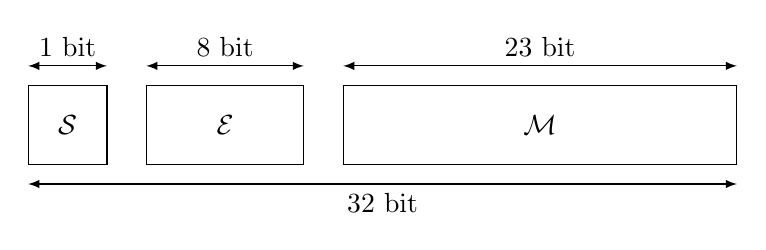
\begin{tikzpicture}
			\draw (0, 0) rectangle +(1, 1)  node[midway] {$\mathcal{S}$};
			\draw (1.5, 0) rectangle +(2, 1)  node[midway] {$\mathcal{E}$};;
			\draw (4, 0) rectangle +(5, 1)  node[midway] {$\mathcal{M}$};
			\draw[latex-latex] (0,1.25) -- +(1,0) node[midway,above]{1 bit};
			\draw[latex-latex] (1.5,1.25) -- +(2,0) node[midway,above]{8 bit};
			\draw[latex-latex] (4,1.25) -- +(5,0) node[midway,above]{23 bit};
			\draw[latex-latex] (0,-.25) -- +(9,0) node[midway,below]{32 bit};
		\end{tikzpicture}
		\begin{equation*}
			x = (-1)^\mathcal{S} \times 2^{\mathcal{E}-2^7} \times \left(1+\frac{\mathcal M}{2^{23}}\right).
		\end{equation*}
	\end{center}
	And yet...
	\begin{minted}{python}
# let's play with floats:
x = 2.5e7  # S=0, E=151, M=4111392
y = x - 3.25e-2
	\end{minted}
	This is a powerful abstraction!
\end{frame}

\begin{frame}{Design by contract (i.e., abstraction by specification)}
	\vspace*{1em}
	\begin{columns}
	\column{.5\linewidth}
	\parskip=1em
	The ``design by contract" approach prescribes that developers should define formal(?), precise(?) and verifiable(?) interface specifications for software components (functions, classes, modules, programs, etc). 
	
	The ``contract'' is the following: $P \land I \implies Q \land I$ ($\land$ side effects). Generally, $\lnot (P \land I)\implies \text{errors}$, but it is not necessarily true in all cases (and it does not have to be). 
	
	\textbf{Notice that this does not say how to get from $P\land I$ to $Q\land I$.} This is thus mostly useful for the programmer (and the user).
	
	\column{.5\linewidth}
	\begin{center}
		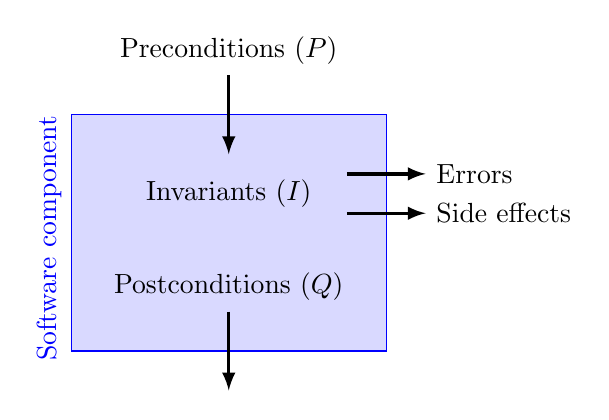
\begin{tikzpicture}
			\draw[blue,fill=blue!15] (0, 0) rectangle +(4, 3);
			\draw[blue]  (0, -.25) node[anchor=south west,rotate=90]{Software component};
			\draw[-latex,very thick] (2, 3.5) node[above]{Preconditions ($P$)}-- +(0, -1);
			\draw[-latex,very thick] (2, 0.5) node[above]{Postconditions  ($Q$)}-- +(0, -1);
			\draw[-latex,very thick] (3.5, 2.25) -- +(1, 0) node[right]{Errors};
			\draw[-latex,very thick] (3.5, 1.75) -- +(1, 0) node[right]{Side effects};
			\draw (2, 2) node{Invariants ($I$)};
		\end{tikzpicture}
	\end{center}
	\vspace*{1em}
	+ Eventual performances guarantees.
	\end{columns}
\end{frame}

\begin{frame}
	\vspace*{1em}
	\begin{columns}
		\column{.5\linewidth}
		\begin{itemize}
			\item The \textbf{preconditions} are predicates that must be true before the execution of the component (it generally boils down to the type of the inputs and their respective domains). It must be guaranteed by \textbf{the caller}. If a precondition is violated, the effect becomes undefined.
			\item The \textbf{postconditions} are predicates that must be true after execution (if the preconditions are true), which is guaranteed by the \textbf{callee}.
			\item The \textbf{invariants} are predicates that must be true before and after execution. This is guaranteed by the caller \textbf{and} the callee (but mostly the later).
		\end{itemize}
		
		\column{.4\linewidth}
		\begin{center}
			\includegraphics[width=\linewidth]{im/meme-prepost}
		\end{center}
	\end{columns}
\end{frame}

\begin{frame}
	Example (abs?) + Side effects + errors.
\end{frame}

\begin{frame}{Documentation}
	docstring and generation?
\end{frame}

\begin{frame}{Testing}
	\begin{itemize}
		\item Test-driven dev
		\item regression/integration/whatever kind of tests
		\item Setup/stimuly/verify/teardown.
		\item Test limit of the domains.
		\item Factory?
	\end{itemize}
\end{frame}

\begin{frame}{Error handling (\textit{exceptions})}
	content...
\end{frame}

\begin{frame}{Data structures}
Other example of abstract data types (list, queue, dictionary, etc).
Note: don't forget $\mathcal O(N)$.
\end{frame}

 \section{POO and POO in Python}
 
 \begin{frame}{What is POO?}
 	\begin{itemize}
 		\item ADT (and internal representation. Example: a molecule and its atoms.
 		\item Methods (CRUDs)  + encapsulation (private/public?).
 		\item Instance of a \textbf{class} + methods.
 	\end{itemize}
 \end{frame}
 
 \section{Organization of a Python project}
 
 \begin{frame}
 	\begin{itemize}
 		\item typing and linting
 		\item Use git
 		\item Don't reinvent the wheel (\textit{battery (already) included})
 		\item README \& LICENSE
 		\item packages (\texttt{import stuff})
 		\item Project (\texttt{pyproject.toml})
 		\item virtualenv
 	\end{itemize}
 \end{frame}

\end{document}